\section{Proofs for Expressiveness Upper Bounds  (\Cref{sec:improved_upper_bounds})}\label{appsec:proofs_transformer_upperbound}


The main technical theorems we will prove in this section are \Cref{thm:iterated_addition_in_AC0,thm:iterated_addition_in_TC0}. Their proofs can be found in \Cref{appsec:AC0_upper_bound,appsec:TC0_upper_bound} respectively.  

Recall $\psi_{e,s}:\Floating_{e,s}\to \{0,1\}^{e+2s+1}$ is the binary representation of floating point with $e$-bit exponent and $2s$-bit precision.
\begin{theorem}\label{thm:iterated_addition_in_AC0}
%Adding $n$ floating point numbers with constantly many bits of exponents and precision and iterative rounding with is in $\AC^0$.
For any fixed $e\in\mathbb{N},s\in\mathbb{N}^+$, $\sumes:(\Floating_{e,s})^n \to \Floating_{e,s}$ has $\AC^0$ circuits.
 
 In detail, there is a family of $\AC^0$ circuits $\{C_n\}$ such that for all $x_1,\ldots,x_n \in \Floating_{e,s}$, it holds that 
	\begin{equation}
		C_n(\psi_{e,s}(x_1)\|\dots\|\psi_{e,s}(x_n)) = \psi_{e,s}(\sumes(x_1,\dots,x_n))
	\end{equation}
\end{theorem}

\begin{theorem}\label{thm:iterated_addition_in_TC0}
%Adding $n$ floating point numbers with constantly many bits of exponents and precision and iterative rounding with is in $\AC^0$.
For $s(n) = O(\poly(n))$, $\mathsf{sum}_{0,s(n)}:(\Floating_{0,s(n)})^n \to \Floating_{0,s(n)}$ has $\TC^0$ circuits.
 
 In detail, there is a family of $\TC^0$ circuits $\{C_n\}$ such that for all $x_1,\ldots,x_n \in \Floating_{0,s(n)}$, it holds that 
	\begin{equation}
		C_n(\psi_{0,s(n)}(x_1)\|\dots\|\psi_{0,s(n)}(x_n)) = \psi_{0,s(n)}(\sumes(x_1,\dots,x_n))
	\end{equation}
\end{theorem}

With \Cref{thm:iterated_addition_in_AC0,thm:iterated_addition_in_TC0} ready, \Cref{thm:AC0_upper_bound,thm:TC0_upper_bound} are standard (e.g., see proof of Theorem 4 in \citet{liu2022transformers}) and thus are omitted.




\subsection{Proofs for \Cref{thm:iterated_addition_in_AC0}}\label{appsec:AC0_upper_bound}
\begin{definition}[Total Order]
	A total order $\le$ on some set $X$ is a binary relationship satisfying that for all $a,b,c\in X$:
	\begin{enumerate}
		\item $a\le a$ (reflexive)
		\item $a\le b$, $b\le c \implies a\le c$ (transitive)
		\item $a\le b$, $b\le a \implies a =b$ (antisymmetric)
		\item $a\le b$ or $b\le a$. (total)
	\end{enumerate}
\end{definition}
\begin{definition}[Ordered Automaton]\label{defi:ordered_automaton}
	We say an automaton $\gA = (\Sigma,Q,\delta)$ is \emph{ordered} if and only if there exists a total order $\le$ on $Q$ and for all $\sigma\in\Sigma$, $\delta(\cdot,\sigma)$ preserves the order, that is,  $$\forall q,q'\in Q, \quad q\ge q' \implies \delta(q,\sigma)\ge \delta(q',\sigma).$$
\end{definition}

\begin{theorem}\label{thm:ordered_automata_counter_free}
	All ordered automata are counter-free. Languages recognizable by any ordered automata belong to $\AC^0$.
\end{theorem}

\begin{proof}[Proof of \Cref{thm:ordered_automata_counter_free}]
	To show an ordered automaton $\gA = (\Sigma,Q,\delta)$ is counter-free, it suffices to its transformation semigroup is group-free, or aperiodic. We first recall the definition of aperiodic semigroups~\Cref{lem:aperiodic}. Let $\pi_w:Q\to Q, \pi_w(q)\triangleq\delta(q,w)$ be the transformation induced by word $w\in\Sigma^*$. Transformation semigroup of $\gA$ is aperiodic iff for any $w\in\Sigma^*$, there exists $k\in\mathbb{N}$, such that $(\pi_w)^k = (\pi_w)^{k+1}$. 
		
	
	Now  We claim for any $q\in Q$, there is $k\in\mathbb{N}$, such that $(\pi_w)^k(q) = (\pi_w)^{k+1}(q)$. Since $Q$ is finite, this implies that there exists $k\in\mathbb{N}$, such that $(\pi_w)^k = (\pi_w)^{k+1}$ and thus the transformation semigroup of $\gA$ is aperiodic. First, note that $\gA$ is ordered, we know $\pi_\sigma$ is order-preserving for all $\sigma\in \Sigma$. Let $w = \overline{w_1\cdots w_n}$ where $|w|=n$, we have $\pi_w = \pi_{w_1}\circ \cdots \circ \pi_{w_n}$ is also order-preserving and thus for all $q\ge q'\in Q$, $\pi_w(q)\ge \pi_w(q')$. Then we proceed by three cases for each $q\in Q$: 
	\begin{enumerate}
		\item $ \pi_w(q)=q$. In this case, it suffices to take $k=0$;
		\item $\pi_w(q)\ge q$. Since $\pi_w$ is order-preserving, we know for any $k\in \mathbb{N}$, $(\pi_w)^{k+1}(q)\ge (\pi_w)^{k}(q)$. Since $Q$ is finite, there must exist some $k\in \mathbb{N}$ such that $(\pi_w)^{k+1}(q)= (\pi_w)^{k}(q)$.
		\item $\pi_w(q)\le q$. Same as the case of $\pi_w(q)\ge q$.
	\end{enumerate}

	Since $\ge$ is a total order, at least one of the three cases happens. This concludes the proof.
	
	The second claim follows directly from \Cref{thm:counter_free_language_three_characterization}.
\end{proof}

For any $e,s\in\mathbb{N}$, iterated addition on floating point numbers with $e$-bit exponent and $s$-bit significand $\Floating_{e,s}$ can be viewed $\gA_{e,s} = (\Floating_{e,s},\Floating_{e,s}, \delta_{+})$.
\begin{theorem}\label{thm:floating_point_is_ordered_automaton}
Automaton $\gA_{e,s} = (\Floating_{e,s},\Floating_{e,s}, \delta_{+})$ is ordered, where $\delta_+(x,y) \triangleq \rdes{x+y}$ for any $x,y\in\Floating_{e,s}$.
\end{theorem}

\begin{proof}[Proof of \Cref{thm:floating_point_is_ordered_automaton}]
	The total order we use for $\Floating_{e,s}$ as the state space of automaton $\gA$ coincides with the usual order $\le$ on $\mathbb{R}$. Recall the rounding operation is defined as $\rdes{x}\in \argmin_{x'\in \Floating_{e,s} \abs{x-x'}}$, which means rounding operation is order preserving, that is, for any $x\ge x'\in\Floating_{e,s}$, $\rdes{x}\ge \rdes{x'}$. Thus for any $x,x',y\in\Floating_{e,s}$ with $x\le x'$, it holds that $\delta_+(x,y) = \rdes{x+y}\ge \rdes{x'+y} = \delta_+(x',y) $. Thus $\gA_{e,s}$ is ordered.
\end{proof}

The following theorem \Cref{thm:iterated_addition_in_AC0} is a direct consequence of \Cref{thm:floating_point_is_ordered_automaton}.

\subsection{Proofs for \Cref{thm:iterated_addition_in_TC0}}\label{appsec:TC0_upper_bound}


	We first claim that the following algorithm \Cref{alg:gridworld} correctly computes $\mathsf{sum}_{0,s(n)}$ over $n$ numbers in $\Floating_{0,s(n)}$.
	
\begin{lemma}\label{lem:TC0_gridworld_algorithm_correct}
	\Cref{alg:gridworld} outputs $\mathsf{sum}_{0,s(n)}(x_1,\ldots,x_n)$ for all $n\in\mathbb{N}^+$ and $x_1,\ldots,x_n\in\Floating_{0,s(n)}$. 
\end{lemma}

\begin{proof}[Proof of \Cref{lem:TC0_gridworld_algorithm_correct}]
Note that $y_{-2}=0$, $[y_{-1}+y_0]_{0,s(n)} = \sign(x_1) \cdot B_{s(n)}$, and $[\sign(x_1) \cdot B_{s(n)} + y_1]_{0,s(n)} = x_1$, thus we conclude $\mathsf{sum}_{0,s(n)}(x_1,\ldots,x_n) = \mathsf{sum}_{0,s(n)}(y_{-2},y_{-1},y_0,y_1,\ldots,y_n)$. 
Without loss of generality, we can assume that $x_1>0$. Therefore $S_{-2} = 0, S_{-1} = B_{s(n)}$, and $S_{0} = 2B_{s(n)}$, which further implies that $L_{-2}\le 0$ and $U_{-2}\ge 2 B_{s(n)}$. This ensures $i^*$ is always well-defined. For convenience we use $H_i$ to denote $\mathsf{sum}_{0,s(n)}(y_{-2},y_{-1},y_0,y_1,\ldots,y_{i-1})$ in the rest of this proof.

Now we claim either $S_{i^*} = L_{i^*}$ or $S_{i^*} = U_{i^*}$. By definition of $i^*$, if neither of these two equalities happen, we have that $i^*\le n-1$, $U_{i^*}= U_{i^*+1}$, and $L_{i^*}= L_{i^*+1}$, which contradicts with the maximality of $i^*$ since $U_{i^*+1} - L_{i^*+1} = U_{i^*} - L_{i^*}\ge 2B_{s(n)}$. Without loss of generality, we assume $S_{i^*} = L_{i^*}$ and the analysis for the other case  is almost the same. Now we claim that for all $i>i^*$, no negative overflow happens at position $i$, that is, $H_i+ y_i\ge -B_{s(n)}$.

We will prove this claim for two cases respectively depending on whether there exists some $i^*<j<i$ such that $\mathsf{sum}_{0,s(n)}(y_{-2},y_{-1},y_0,y_1,\ldots,y_{j}) = B_{s(n)}$.  The first case is such $j$ does not exist. Then neither positive or negative overflow happens through $i^*$ to $i$, and thus 
\begin{align}
H_{i-1} + y_i 
= H_{i^*} + (S_i-S_{i^*})
\ge  H_{i^*} 
\ge -B_{s(n)}.
\end{align}

If such $j$ exists, we let $j^*$ to be the maximum of such $j$. Then neither positive or negative overflow happens through $j^*$ to $i$. Due to the optimality of $i^*$, we know that for all $i,j\ge i^*$, $ \abs{S_{i}-S_{j}}<   2B_{s(n)}<$. Thus
\begin{align}
H_{i-1} + y_i 
= H_{j^*} + (S_i-S_{j^*})
\ge  B_{s(n)} - 2B_{s(n)} 
\ge -B_{s(n)}.
\end{align} 

Now we claim $H_{k^*} = B_{s(n)}$. Because there is no negative overflow between $i^*$ and $k^*$, we have that $H_{k^*}- H_{i^*} \ge S_{k^*}-S_{i^*}\ge 2B_{s(n)}$ and the fist inequality is only strict when positive overflow happens at some $i^*\le j\le k^*$. If there is no such $j$, then $B_{s(n)}\ge H_{k^*}\ge H_{i^*}+2B_{s(n)}\ge B_{s(n)}$ and thus $H_{k^*} = B_{s(n)}$. Otherwise such $j$ exists and $j^*$ be the maximum of such $j$. Then $H_{k^*}\ge  H_{j^*} + (S_{k^*}-S_{j^*}) \ge B_{s(n)} + (S_{k^*}-S_{j^*})\ge B_{s(n)}$, where the last inequality is due to the optimality of $k^*$. Thus in both cases we conclude that $H_{k^*} = B_{s(n)}$. 

Finally we will show there is neither negative or positive overflow from $k^*+1$ to $n$ and thus $H_n = H_{k^*} + S_n-S_{k^*}$, which would justify the correctness of the algorithm. We have already shown there is no negative overflow. Suppose there is a positive overflow at some $j>k^*$ in the sense that $H_{j-1}+y_j\ge B_{s(n)}$ and we let $j^*$ be the first positive overflow after $k^*$. By definition of $j^*$, there is neither positive and negative overflow between $k^*+1$ and $j^*$ and thus $H_{j^*-1}+y_{j^*} = H_{k^*} + (S_{j^*} - S_{k^*})\le H_{k^*}=B_{s(n)}$, which is contradictory to the assumption that there is a positive overflow at $j^*$. This concludes the proof. 
\end{proof}


	
\begin{algorithm}
\caption{$\AC^0$ algorithm for iterative addition for poly-precision floating point numbers}\label{alg:gridworld}
\begin{algorithmic}[1]

\Require Integer $n\in\mathbb{N}^+$, $s(n)=O(\poly(n))$. Floating numbers $x_1,\ldots, x_n\in \Floating_{0,s(n)}$.
\Ensure $\mathsf{ans} = \mathsf{sum}_{0,s(n)}(x_1,\ldots,x_n)\in\Floating_{0,s(n)}$.

\State   $y_{-2}\gets 0, y_{-1},y_{0} \gets \sign(x_1) \cdot B_{s(n)}$, $y_1 \gets x_1 -\sign(x_1) \cdot B_{s(n)}$, $y_i \gets x_i, \forall i\in\{2,\ldots,n\}$;
\State   $S_i\gets \sum_{j=0}^i y_j,\ \forall i\in\{-2,\ldots,n\}$;
\State   $U_i \gets \max_{i\le j\le n} S_j, L_i \gets \min_{i\le j\le n} S_j,\ \forall i\in\{-2,\ldots, n\}$;
\State $i^*  \gets \max \{-2\le i\le n\mid U_i-L_i\ge 2B_{s(n)}\}$;
\If{$S_{i^*} = U_{i^*}$}
\State   $k^*  \gets \max\{i^*\le k\le n\mid S_{k} = L_{i^*}\}$;
\State   $O  \gets -B_{s(n)}$;
\Else
\State   $k^*  \gets \max\{i^*\le k\le n\mid S_{k} = U_{i^*}\}$;
\State   $O  \gets B_{s(n)}$;
\EndIf
\State $\mathsf{ans}\gets O + S_{n} -  S_{k^*}$.
\end{algorithmic}
\end{algorithm}

\begin{proof}[Proof of \Cref{thm:TC0_upper_bound}]
It suffices to show that \Cref{alg:gridworld} can be implemented by a family of $\TC^0$ circuits since \Cref{lem:TC0_gridworld_algorithm_correct} guarantees the correctness of \Cref{alg:gridworld}. We can treat all the fixed-point floating numbers in the \Cref{alg:gridworld} as integers with a suitable rescaling, which is $2^{s(n)}$. Since both sorting and adding $n$ binary integers with polynomial bits have $\TC^0$ circuits, each line in \Cref{alg:gridworld} can be implemented by an $\TC^0$ circuits (for all indexes $i$ simultaneously if there is any).
\end{proof}
	 
\begin{figure}[t]
\begin{center}
\vspace{-1.5cm}
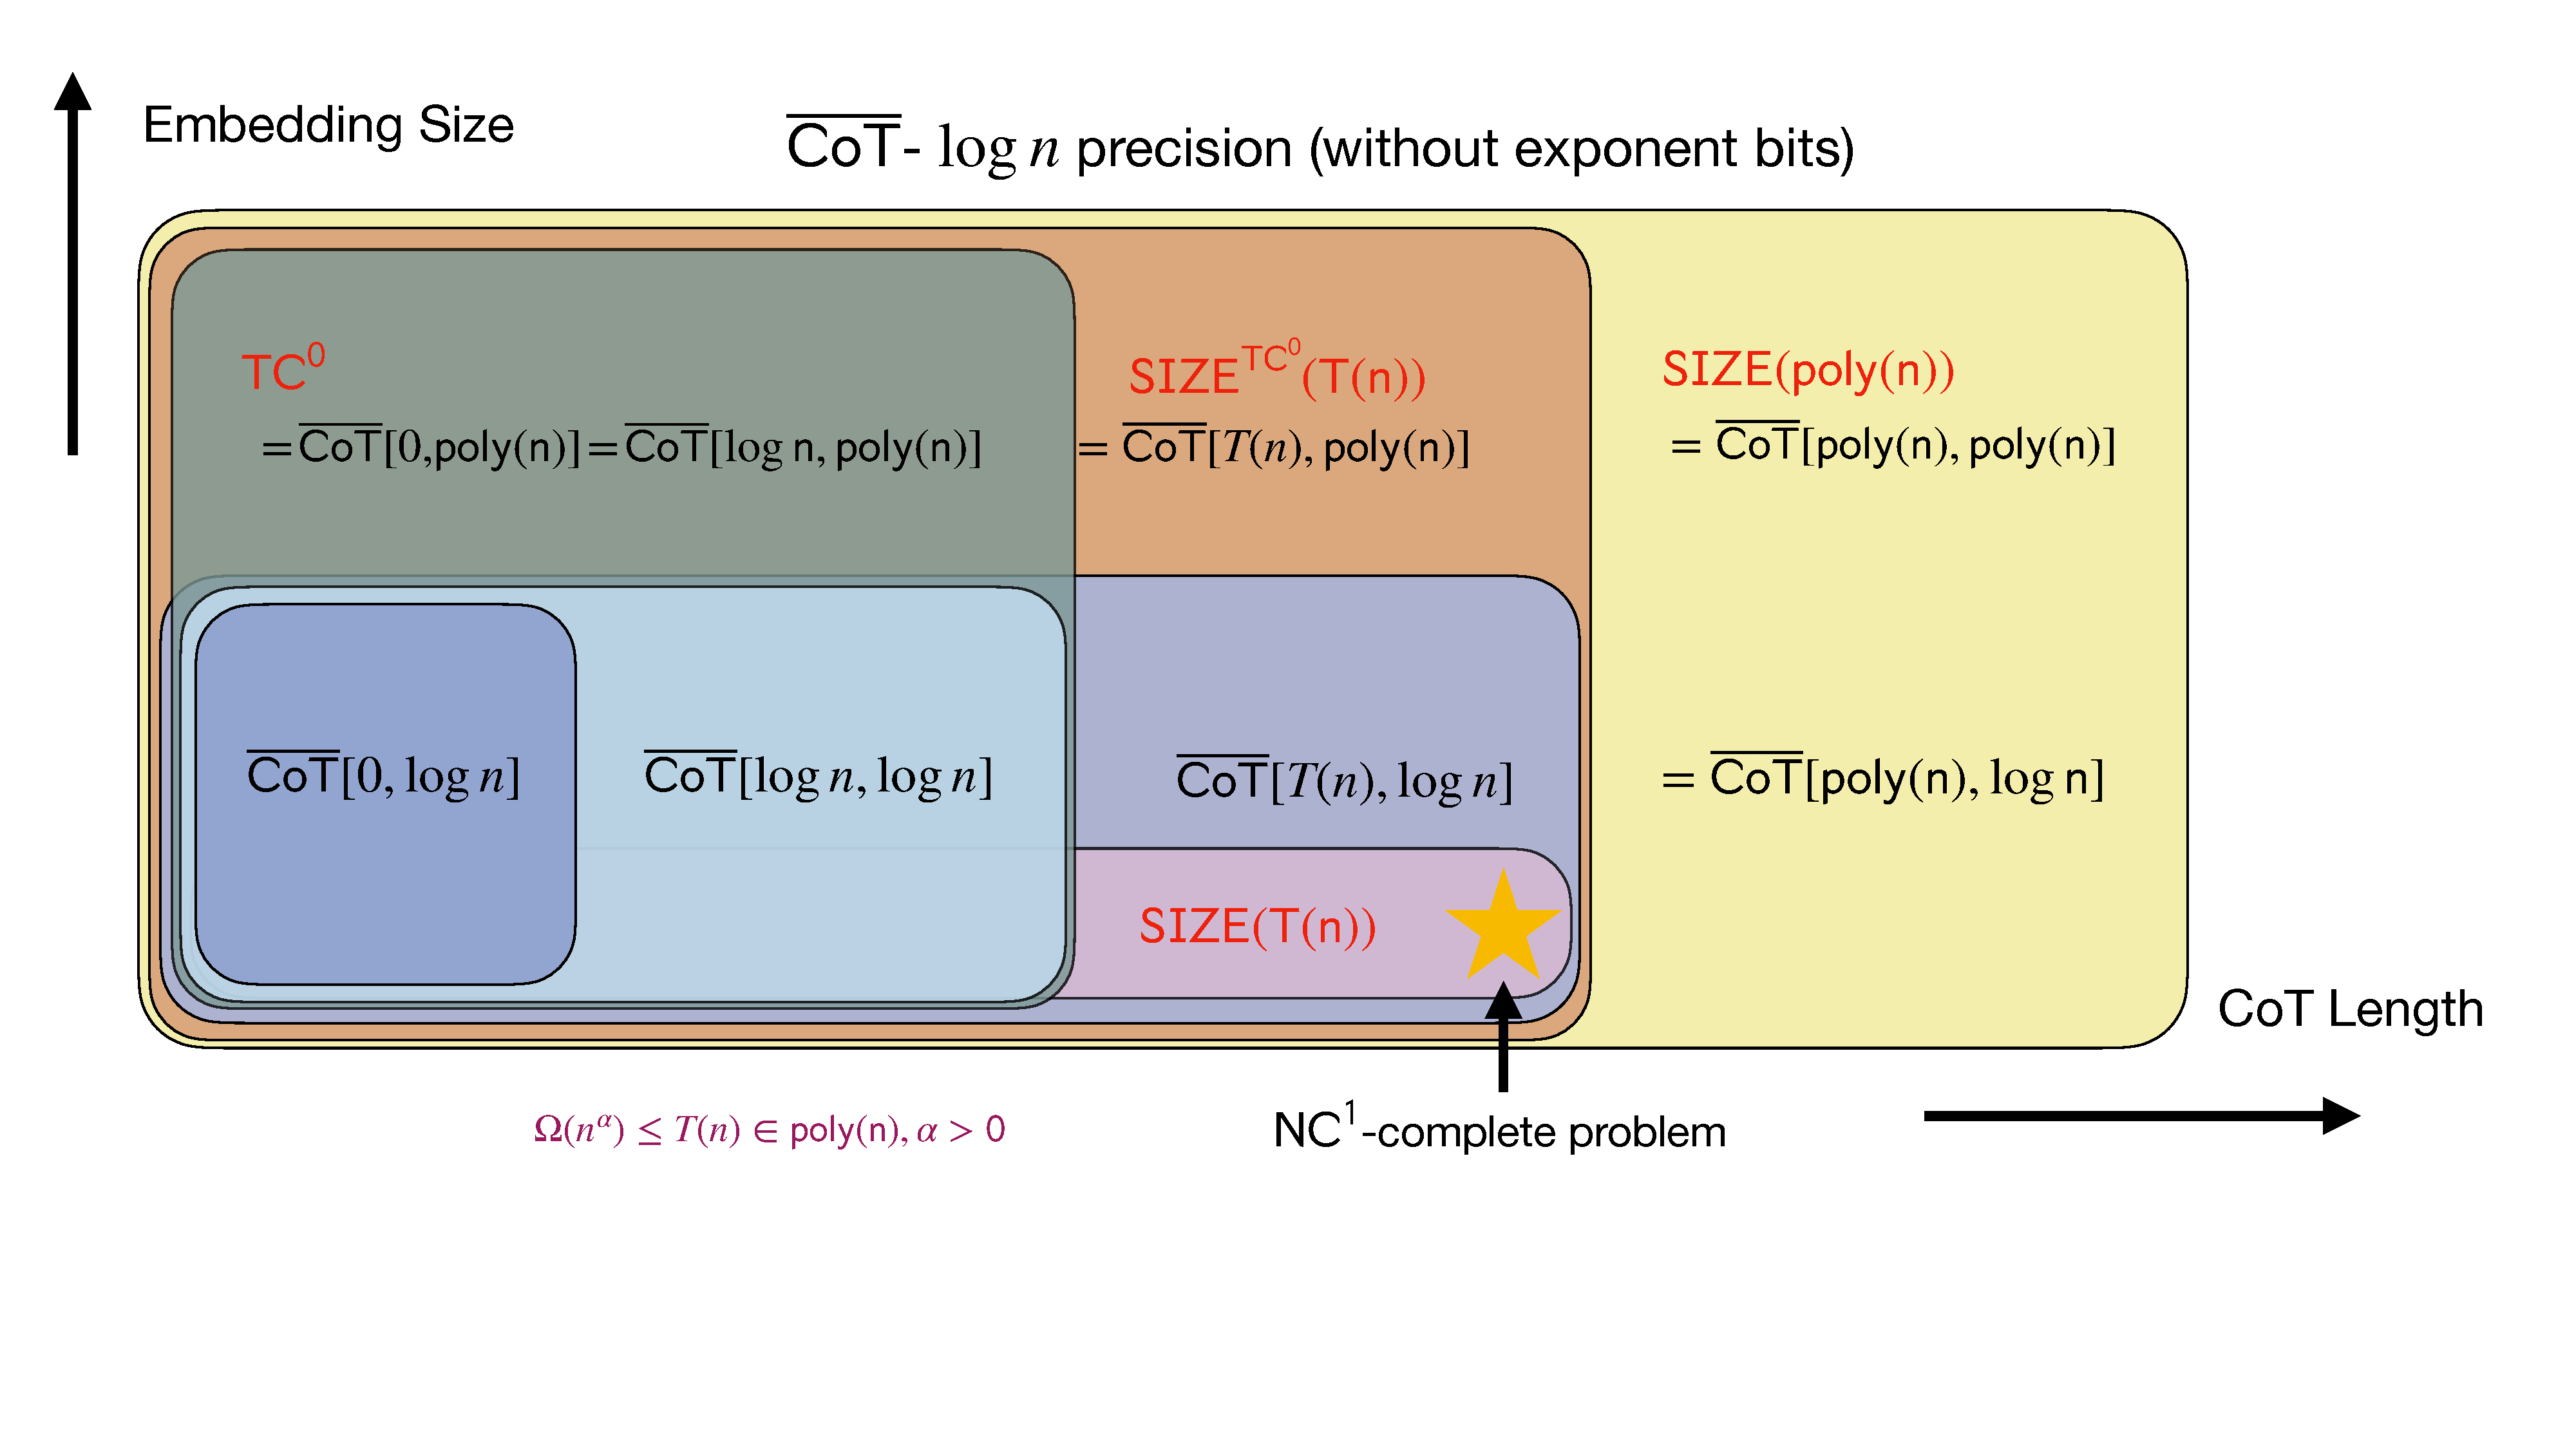
\includegraphics[width=1.1\textwidth]{figures/cot_diagram_log.pdf}
\vspace{-2cm}
\caption{Relationship diagram between \cot complexity class with different embedding sizes $d(n)$ and CoT lengths $T(n)$. We fix the precision to be $\log(n)$ and the number of exponents bit as $0$. This is the counterpart of its finite precision version~\Cref{fig:cot_diagram_constant} }\label{fig:cot_diagram_log}
\end{center}
\end{figure}
